% Created by tikzDevice version 0.12.3 on 2020-09-22 19:19:05
% !TEX encoding = UTF-8 Unicode
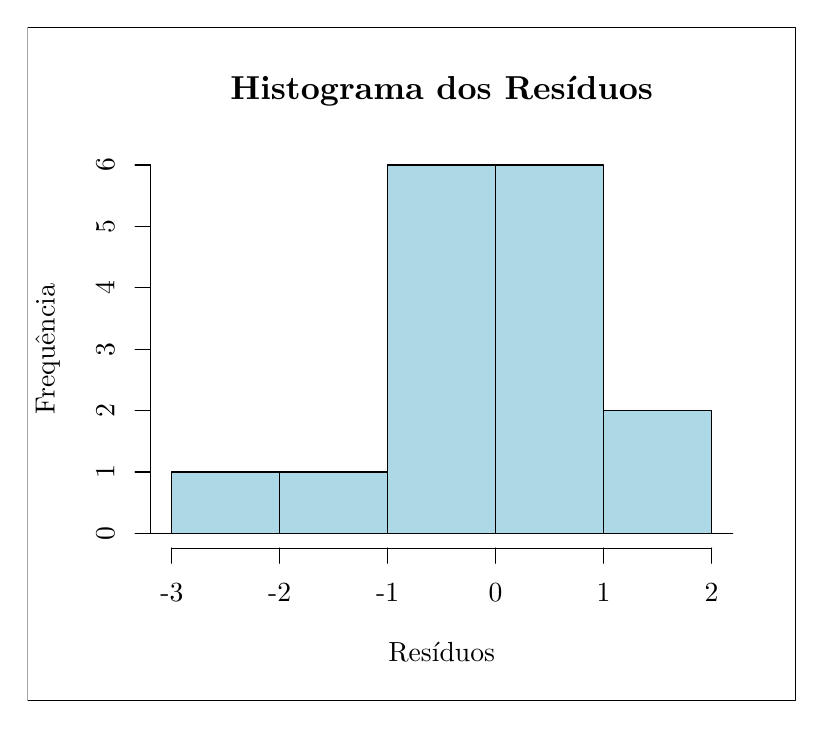
\begin{tikzpicture}[x=1pt,y=1pt, scale=0.9]
\definecolor{fillColor}{RGB}{255,255,255}
\path[use as bounding box,fill=fillColor,fill opacity=0.00] (0,0) rectangle (308.44,270.16);
\begin{scope}
\path[clip] (  0.00,  0.00) rectangle (308.44,270.16);
\definecolor{drawColor}{RGB}{0,0,0}

\node[text=drawColor,anchor=base,inner sep=0pt, outer sep=0pt, scale=  1.20] at (166.22,241.42) {\bfseries Histograma dos Resíduos};

\node[text=drawColor,anchor=base,inner sep=0pt, outer sep=0pt, scale=  1.00] at (166.22, 15.60) {Resíduos};

\node[text=drawColor,rotate= 90.00,anchor=base,inner sep=0pt, outer sep=0pt, scale=  1.00] at ( 10.80,141.08) {Frequência};
\end{scope}
\begin{scope}
\path[clip] (  0.00,  0.00) rectangle (308.44,270.16);
\definecolor{drawColor}{RGB}{0,0,0}

\path[draw=drawColor,line width= 0.4pt,line join=round,line cap=round] ( 57.87, 61.20) -- (274.57, 61.20);

\path[draw=drawColor,line width= 0.4pt,line join=round,line cap=round] ( 57.87, 61.20) -- ( 57.87, 55.20);

\path[draw=drawColor,line width= 0.4pt,line join=round,line cap=round] (101.21, 61.20) -- (101.21, 55.20);

\path[draw=drawColor,line width= 0.4pt,line join=round,line cap=round] (144.55, 61.20) -- (144.55, 55.20);

\path[draw=drawColor,line width= 0.4pt,line join=round,line cap=round] (187.89, 61.20) -- (187.89, 55.20);

\path[draw=drawColor,line width= 0.4pt,line join=round,line cap=round] (231.23, 61.20) -- (231.23, 55.20);

\path[draw=drawColor,line width= 0.4pt,line join=round,line cap=round] (274.57, 61.20) -- (274.57, 55.20);

\node[text=drawColor,anchor=base,inner sep=0pt, outer sep=0pt, scale=  1.00] at ( 57.87, 39.60) {-3};

\node[text=drawColor,anchor=base,inner sep=0pt, outer sep=0pt, scale=  1.00] at (101.21, 39.60) {-2};

\node[text=drawColor,anchor=base,inner sep=0pt, outer sep=0pt, scale=  1.00] at (144.55, 39.60) {-1};

\node[text=drawColor,anchor=base,inner sep=0pt, outer sep=0pt, scale=  1.00] at (187.89, 39.60) {0};

\node[text=drawColor,anchor=base,inner sep=0pt, outer sep=0pt, scale=  1.00] at (231.23, 39.60) {1};

\node[text=drawColor,anchor=base,inner sep=0pt, outer sep=0pt, scale=  1.00] at (274.57, 39.60) {2};

\path[draw=drawColor,line width= 0.4pt,line join=round,line cap=round] ( 49.20, 67.12) -- ( 49.20,215.04);

\path[draw=drawColor,line width= 0.4pt,line join=round,line cap=round] ( 49.20, 67.12) -- ( 43.20, 67.12);

\path[draw=drawColor,line width= 0.4pt,line join=round,line cap=round] ( 49.20, 91.77) -- ( 43.20, 91.77);

\path[draw=drawColor,line width= 0.4pt,line join=round,line cap=round] ( 49.20,116.42) -- ( 43.20,116.42);

\path[draw=drawColor,line width= 0.4pt,line join=round,line cap=round] ( 49.20,141.08) -- ( 43.20,141.08);

\path[draw=drawColor,line width= 0.4pt,line join=round,line cap=round] ( 49.20,165.73) -- ( 43.20,165.73);

\path[draw=drawColor,line width= 0.4pt,line join=round,line cap=round] ( 49.20,190.39) -- ( 43.20,190.39);

\path[draw=drawColor,line width= 0.4pt,line join=round,line cap=round] ( 49.20,215.04) -- ( 43.20,215.04);

\node[text=drawColor,rotate= 90.00,anchor=base,inner sep=0pt, outer sep=0pt, scale=  1.00] at ( 34.80, 67.12) {0};

\node[text=drawColor,rotate= 90.00,anchor=base,inner sep=0pt, outer sep=0pt, scale=  1.00] at ( 34.80, 91.77) {1};

\node[text=drawColor,rotate= 90.00,anchor=base,inner sep=0pt, outer sep=0pt, scale=  1.00] at ( 34.80,116.42) {2};

\node[text=drawColor,rotate= 90.00,anchor=base,inner sep=0pt, outer sep=0pt, scale=  1.00] at ( 34.80,141.08) {3};

\node[text=drawColor,rotate= 90.00,anchor=base,inner sep=0pt, outer sep=0pt, scale=  1.00] at ( 34.80,165.73) {4};

\node[text=drawColor,rotate= 90.00,anchor=base,inner sep=0pt, outer sep=0pt, scale=  1.00] at ( 34.80,190.39) {5};

\node[text=drawColor,rotate= 90.00,anchor=base,inner sep=0pt, outer sep=0pt, scale=  1.00] at ( 34.80,215.04) {6};
\end{scope}
\begin{scope}
\path[clip] ( 49.20, 61.20) rectangle (283.24,220.96);
\definecolor{drawColor}{RGB}{0,0,0}
\definecolor{fillColor}{RGB}{173,216,230}

\path[draw=drawColor,line width= 0.4pt,line join=round,line cap=round,fill=fillColor] ( 57.87, 67.12) rectangle (101.21, 91.77);

\path[draw=drawColor,line width= 0.4pt,line join=round,line cap=round,fill=fillColor] (101.21, 67.12) rectangle (144.55, 91.77);

\path[draw=drawColor,line width= 0.4pt,line join=round,line cap=round,fill=fillColor] (144.55, 67.12) rectangle (187.89,215.04);

\path[draw=drawColor,line width= 0.4pt,line join=round,line cap=round,fill=fillColor] (187.89, 67.12) rectangle (231.23,215.04);

\path[draw=drawColor,line width= 0.4pt,line join=round,line cap=round,fill=fillColor] (231.23, 67.12) rectangle (274.57,116.42);
\end{scope}
\begin{scope}
\path[clip] (  0.00,  0.00) rectangle (308.44,270.16);
\definecolor{drawColor}{RGB}{0,0,0}

\path[draw=drawColor,line width= 0.4pt,line join=round,line cap=round] ( 57.87, 61.20) -- (274.57, 61.20);

\path[draw=drawColor,line width= 0.4pt,line join=round,line cap=round] ( 57.87, 61.20) -- ( 57.87, 55.20);

\path[draw=drawColor,line width= 0.4pt,line join=round,line cap=round] (101.21, 61.20) -- (101.21, 55.20);

\path[draw=drawColor,line width= 0.4pt,line join=round,line cap=round] (144.55, 61.20) -- (144.55, 55.20);

\path[draw=drawColor,line width= 0.4pt,line join=round,line cap=round] (187.89, 61.20) -- (187.89, 55.20);

\path[draw=drawColor,line width= 0.4pt,line join=round,line cap=round] (231.23, 61.20) -- (231.23, 55.20);

\path[draw=drawColor,line width= 0.4pt,line join=round,line cap=round] (274.57, 61.20) -- (274.57, 55.20);

\path[draw=drawColor,line width= 0.4pt,line join=round,line cap=round] ( 49.20, 67.12) -- ( 49.20,215.04);

\path[draw=drawColor,line width= 0.4pt,line join=round,line cap=round] ( 49.20, 67.12) -- ( 43.20, 67.12);

\path[draw=drawColor,line width= 0.4pt,line join=round,line cap=round] ( 49.20, 91.77) -- ( 43.20, 91.77);

\path[draw=drawColor,line width= 0.4pt,line join=round,line cap=round] ( 49.20,116.42) -- ( 43.20,116.42);

\path[draw=drawColor,line width= 0.4pt,line join=round,line cap=round] ( 49.20,141.08) -- ( 43.20,141.08);

\path[draw=drawColor,line width= 0.4pt,line join=round,line cap=round] ( 49.20,165.73) -- ( 43.20,165.73);

\path[draw=drawColor,line width= 0.4pt,line join=round,line cap=round] ( 49.20,190.39) -- ( 43.20,190.39);

\path[draw=drawColor,line width= 0.4pt,line join=round,line cap=round] ( 49.20,215.04) -- ( 43.20,215.04);
\end{scope}
\begin{scope}
\path[clip] ( 49.20, 61.20) rectangle (283.24,220.96);
\definecolor{drawColor}{RGB}{0,0,0}

\path[draw=drawColor,line width= 0.4pt,line join=round,line cap=round] ( 49.20, 67.12) -- (283.24, 67.12);
\end{scope}
\begin{scope}
\path[clip] (  0.00,  0.00) rectangle (308.44,270.16);
\definecolor{drawColor}{RGB}{0,0,0}

\path[draw=drawColor,line width= 0.4pt,line join=round,line cap=round] (  0.00,  0.00) --
	(308.44,  0.00) --
	(308.44,270.16) --
	(  0.00,270.16) --
	(  0.00,  0.00);
\end{scope}
\end{tikzpicture}
